%% Hello emacs, this is -*- latex -*-
\typeout{ ====================================================================}
\typeout{ This is file introducao.tex, created at 01-Feb-2004 }
\typeout{ Maintained by Andre DOS ANJOS <Andre.dos.Anjos@cern.ch> }
\typeout{ ====================================================================}

\chapter{A Física de Altas Energias}
\label{chap:introducao}

\idx{Física de Partículas} ou \idx{Física de Altas Energias} (do inglês,
\idxeng{High Energy Physics}, comumente abreviado por \eng{HEP}) denomina o
ramo da física que estuda a matéria enquanto formada por partículas
sub-atômicas como elétrons, quarks e prótons, e suas propriedades.

Neste capítulo, introduzimos seus conceitos fundamentais, iniciando com um
breve histórico desta área. O material desta seção encontra-se detalhado em
\cite{partadv}.

%% Advocate: necessário para o leitor entender porquê fala-se que o CERN é
%% o topo de gama neste campo!

\section{Um Pouco de História}

Desde a Antiguidade, as pessoas têm buscado entender o comportamento da
matéria: \textit{- Porque objetos soltos no espaço caem no chão?}, \textit{-
Porque materiais diferentes tem propriedades diferentes?}, e assim por
diante. Outros mistérios incluem a característica do próprio universo onde
habitamos e o comportamento dos corpos celestes. Muitas teorias foram
propostas desde então, a maior parte errada, embora este seja um efeito
colateral da empreitada científica. As teorias físicas na Antiguidade eram
baseadas somente em termos filosóficos e raramente verificadas por testes
experimentais sistemáticos.

Já no início do século XVII, Kepler formulou um modelo do sistema solar
baseado em cinco sólidos platônicos, em uma tentativa de explicar porque as
órbitas dos planetas tinham os tamanhos relativos observados. Seu acesso às
observações acuradas realizadas por outro cientista da época o capacitou
determinar que seu modelo estava inconsistente com as órbitas
observadas. Depois de um esforço heróico de 7 anos, Kepler concluiu que os
planetas não descrevem uma órbita circular, mas elíptica, tendo o Sol em um de
seus focos. Kepler também sugeriu que uma ``força'' emanada do Sol afastaria
os planetas de suas órbitas naturais, levando-os a perseguir uma órbita
elíptica.

Durante este mesmo século, Galileu fez uso, pela primeira vez, de um
``experimento'' no sentido acadêmico da palavra, para validar teorias físicas,
uma idéia-chave no método científico atual. O uso do experimento por Galileu e
sua insistência de que os resultados observados terão sempre que anteceder os
resultados teóricos eliminaram a aceitação de ``dogmas'' e fizeram nascer uma
nova era, onde as idéias científicas eram abertamente discutidas e
rigorosamente testadas.

Dentre outros grandes momentos, em 1687, \idx{Isaac Newton} publicou o
\eng{Principia Mathematica}, detalhando dois compreensivos e bem sucedidos
modelos físicos: a lei do movimento, de onde parte a mecânica clássica; e a
lei da gravidade, que descreve esta força fundamental. Ambas as teorias
concordavam bastante bem com experimentos executados na época. A mecânica
clássica foi exaustivamente estendida por vários outros cientistas que
produziram novas formulações, princípios e resultados.

O início do século XX iniciou uma revolução na Física. As aclamadas teorias
newtonianas mostraram-se incorretas em várias circunstâncias. Não somente a
\idx{Mecânica Quântica} mostrou que as leis do movimento não se confirmavam em
pequenas escalas como, ainda mais inquietante, a relatividade geral mostrou
que o fundo fixo do espaço-tempo, no qual a mecânica newtoniana e a
relatividade especial dependiam, não poderia existir.

Em 1904, Thomson propôs o primeiro modelo atômico, conhecido como
\idx{``Pudim de Ameixas''}\footnote{A existência do átomo tinha sido proposta
em 1808 por Dalton.}. Já em 1905, apenas um ano depois, Einstein formulou a
``Teoria de Relatividade Especial'', unificando espaço e tempo em uma entidade
singular, chamada de espaço-tempo. Em 1915, o próprio estendeu sua teoria de
relatividade especial com a ``Teoria de Relatividade Geral'', substituindo a
lei newtoniana sobre a gravidade. As teorias de Newton e Einstein concordam
para regimes de pouca massa e energia.

Ainda em 1911, Rutherford deduziu a existência de um \idx{núcleo atômico}
compacto, consistindo de cargas positivas chamadas de \idx{prótons}. Para tal,
utilizou-se de um feixe de partículas alfa, emitido por uma fonte radioativa,
uma folha de ouro e um simples detetor feito de Sulfeto de Zinco para testar
sua teoria \cite{halliday}. As partículas alfa, ao baterem no detetor,
marcavam-no (veja a configuração do experimento de Rutherford na
Figura~\ref{fig:rutherford}). Embora não pudesse ver o que ocorria no mundo
sub-atômico, Rutherford podia teorizar, testar sua hipótese e então analisar
os dados experimentais para verificar se seus cálculos estavam corretos. A
única teoria cabível, após seus experimentos, é que o átomo teria que ser
composto por um núcleo compacto e positivo e uma periferia negativamente
carregada de partículas mais leves e menores que aquelas no núcleo.

\begin{figure}
\begin{center}
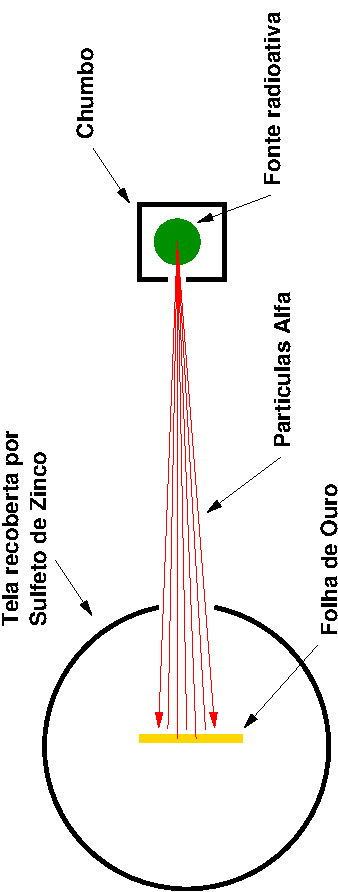
\includegraphics[scale=0.9,angle=-90]{rutherford}
\end{center}
\caption[O \eng{setup} de Rutherford.]{A configuração do experimento de
Rutherford para a constatação de que o núcleo atômico era denso e
positivo. Extraída de \cite{partadv}.}
\label{fig:rutherford}
\end{figure}

Os \idx{nêutrons}, os constituintes nucleares de carga neutra, foram
descobertos em 1932 por Chadwick. Planck e Bohr entre outros físicos
desenvolveram as teorias quânticas para explicar várias anomalias
experimentais, introduzindo o conceito de níveis (ou \idxeng{quanta}) de
energia. Em 1925, Heisenberg e Schrödinger formularam a \idx{Mecânica
Quântica}, que explica as teorias quânticas anteriores. Nesta área, os
resultados de medidas físicas são de natureza inerentemente probabilística. A
teoria modela o cálculo destas probabilidades e, de forma bem-sucedida,
descreve o comportamento da matéria em pequenas escalas.

A mecânica quântica tam\-bém fornece ferramentas te\-ó\-ri\-cas para a
fí\-si\-ca de ma\-té\-ria condensada, que estuda o comportamento físico de
sólidos e líquidos, incluindo fenômenos de cristalização, semi-condutividade e
super-condutividade.

A \idx{Teoria Quântica dos Campos} foi formulada para estender a mecânica
quântica fazendo-a consistente com a relatividade especial, atingindo sua
forma moderna no final dos anos 40 com o trabalho de Feynman, Schwinger,
Tomonaga e Dyson. Eles formularam a \idx{Eletrodinâmica Quântica}, que
descreve a interação eletromagnética.

A teoria quântica dos campos fornece o ferramental de fundo para a fí\-si\-ca
de par\-tí\-cu\-las moderna, que estuda primordialmente as forças elementares
entre as partículas. Em 1954, Yang e Mills desenvolveram uma classe de teorias
de Gauge, introduzindo o \idx{Modelo Atômico Padrão} ou simplesmente
\idx{Modelo Padrão}, que foi completado nos anos 70. O Modelo Padrão descreve
de forma bem-sucedida quase todas as partículas elementares observadas até
hoje e abrange as \idx{forças fundamentais} ``forte'', ``fraca'' e
``eletromagnética'' assim como as partículas de que se compõe toda a matéria
conhecida. O Modelo Padrão não é, no entanto, uma teoria fundamental de todas
a interações existentes na natureza, primariamente por não descrever a
gravidade.

\section{Física de Partículas Moderna}

Embora de grande sucesso, modelando resultados encontrados
ex\-pe\-ri\-men\-tal\-men\-te, o Modelo Pa\-drão nunca foi aceito como uma
teoria completa de física fundamental. Isto acontece por causa de dois
aspectos:

\begin{enumerate}
\item O modelo contém 19 parâmetros livres, como a massa das partículas, que
  precisam ser determinados experimentalmente (e mais outros 10 para massas de
  neutrinos). Estes parâmetros não podem ser calculados independentemente;

\item O modelo não descreve a interação gravitacional;
\end{enumerate}

Desde o complemento do Modelo Padrão, muitos esforços foram travados para
resolver ambos os pontos. Um deles é conhecido como a \idx{Grande Unificação},
do qual muitos aspectos estão bastante longe de serem observados em
laboratório. O bóson de Higgs\index{bóson de Higgs}, que é previsto pelo
modelo padrão, ainda não foi observado até os dias de hoje. Alguns
experimentos, dentre os quais o experimento \idx{ATLAS} (do inglês, \eng{A
Toroidal LHC Apparatus}) no \idx{CERN}, Suíça, estão sendo construído para o
estudo desta física.

\subsection{Aceleradores e Detetores}

De forma parecida a Rutherford, os físicos atuais usam um feixe de partículas
aceleradas para recriar em laboratório condições que permitam o estudo das
interações sub-atômicas que se deseja averiguar. Este feixes podem colidir com
um alvo fixo ou com um outro feixe de partículas, que é acelerado em direção
contrária ao feixe primário. Para visualizar eletronicamente os sub-produtos
de tais interações físicas, utilizam-se múltiplos detetores.

A aceleração das partículas resolve dois problemas que os físicos de hoje
encontram em seus experimentos:

\begin{enumerate}
\item Comprimento de Onda - O comprimento de onda determina a acurácia do que
é possível observar \cite{partadv}.

Uma vez que as par\-tí\-culas tam\-bém apresentam caracte\-rís\-ticas de onda,
não é pos\-sí\-vel obter uma medida acurada usando-se partículas comuns, como
um e\-lé\-tron, na observação de partículas muito pequenas. Um elétron não
serve, nem mesmo, para observar outro elétron. A aceleração da partícula, no
entanto, aumenta seu momento, diminuindo\footnote{O comprimento de onda e o
momento de um corpo são inversamente proporcionais.} seu comprimento de onda e
permitindo que medidas acuradas possam ser tomadas, usando-se partículas
maiores, como léptons.

\item Energia Cinética - Deseja-se, nos experimentos modernos, que o impacto
seja o mais aniquilador possível. Isto é interessante, pois ao se aniquilar
matéria, liberando muita energia, partículas mais massivas e menos estáveis são
geradas. Ao se acelerar uma partícula, aumenta-se sua energia cinética,
tornando a colisão com o alvo mais eficiente (melhor aniquilação).
\end{enumerate}

\subsection{A Aceleração das Partículas}

A aceleração de partículas \index{aceleração de partículas} é um processo
bastante simples: inicialmente devem-se escolher partículas eletricamente
carregadas para um experimento - e\-lé\-trons, pó\-sitrons, pró\-tons,
anti-\-pró\-tons ou íons são utilizados normalmente. As par\-tí\-culas
eletricamente carregadas são posicionadas no interior de um túnel e
aceleradas por pulsos eletromagnéticos\index{pulsos eletromagnéticos}
(e.m). A Figura~\ref{fig:acelera} exemplifica como elétrons possam ser
acelerados: as ondas e.m. aceleram as partículas, pois elementos eletricamente
carregados adquirem força (aceleração) quando envoltos por um campo
eletromagnético.

\begin{figure}
\begin{center}
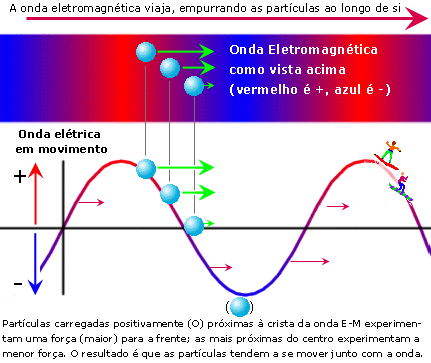
\includegraphics[scale=0.7]{static-wave}
\end{center}
\caption[A aceleração de partículas.]{A aceleração de partículas eletricamente
carregadas usando-se de pulsos e.m.. Extraído de \cite{partadv}.}
\label{fig:acelera}
\end{figure}

Os aceleradores podem ter dois formatos\index{acelerador!tipos}: linear e
circular. Num acelerador linear\index{acelerador!linear}, as partículas são
injetadas em uma extremidade e percorrem uma reta até que colidam com outras
partículas ou com um alvo fixo. A outra possibilidade é ter um acelerador
circular ou
síncrotron\index{acelerador!circular}\index{acelerador!síncrotron|see{acelerador
circular}}. Num acelerador circular, as partículas são injetadas em um ponto
do anel de aceleração e lá permanecem até que tenham adquirido velocidade
suficiente ao experimento a que se destinam. A aceleração circular exige que
ímãs poderosos curvem a trajetória das partículas injetadas. Aceleradores
circulares também permitem que vários experimentos sejam conduzidos em pontos
de sua circunferência, de forma simultânea. Aceleradores circulares possuem
uma desvantagem: quanto maior a energia necessária no centro de impacto, maior
deve ser o perímetro de sua circunferência.

\subsection{Deteção: Vendo o que ocorreu a\-pós a coli\-são}

Depois de um acelerador ter ``bombeado''\ energia suficiente para suas
par\-tí\-culas, estas são colocadas em rota de colisão com um alvo fixo ou,
então, com as partículas de um outro feixe acelerado. Cada uma dessas colisões
forma um \emph{evento} físico. O objetivo dos físicos é isolar cada evento,
coletar dados a seu respeito e verificar se o processo do qual a partícula
participou está de acordo com a teoria que está sendo testada no experimento
em questão.

A análise de cada evento pode ser bastante complexa, já que muitas (sub)
par\-tí\-cu\-las podem ser produzidas. A maioria dessas partículas têm tempo
de vida tão diminuto que viajam por distâncias extremamente curtas, antes de
decaírem em outras partículas, sem deixarem pistas aparentemente detetáveis.

Para procurar esses vários objetos e os produtos de seus decaimentos, os
físicos projetam detetores com multi-componentes, que testam diferentes
aspectos de um evento \cite{d0, cms, atlas-tp, booth}. Cada componente de um
detetor moderno é usado para medir vários parâmetros das partículas
provenientes de um evento, e/ou distinguir os diferentes tipos de objetos
gerados.  Quando todos esses componentes funcionam juntos para detetar um
evento, partículas individuais podem ser distinguidas da multidão para efeito
de análise e o evento original pode ser reconstruído.

Seguindo cada evento, os sistemas de processamento coletam e interpretam a
vasta quantidade de dados dos detetores e apresentam os resultados extrapolados
aos físicos.

Os físicos interessam-se pelos eventos que ocorrem durante ou mesmo depois da
colisão das partículas. Por essa razão, colocam detetores em regiões nas quais
os objetos resultantes daquela interação passarão. Os detetores são construídos
de diferentes maneiras, dependendo do tipo de colisão analisada:

\begin{description}
\item[Alvo fixo] Num experimento envolvendo um alvo fixo, as partículas
produzidas geralmente projetam-se para frente; por isso, os detetores são na
forma de cones e são colocados ao longo da direção do feixe;

\item[Feixes de colisão] Durante um experimento envolvendo feixes em
co\-li\-são, as par\-tí\-cu\-las são espalhadas em todas as direções; assim, o
detetor mais adequado é esférico ou, mais comumente, cilíndrico.
\end{description}

\subsubsection{Composição dos Detetores}

Os detetores modernos são feitos de peças distintas, que testam diferentes
aspectos de um evento. Esses vários componentes são organizados de tal maneira
que os físicos possam obter o máximo de informação sobre as partículas geradas
durante um evento. A Figura~\ref{fig:modern-detect} mostra um diagrama
esquemático de um pequeno detetor cilíndrico moderno. Uma figura humana é
mostrada em escala, indicando a enormidade dos detetores típicos de altas
energias.

\begin{figure}
\begin{center}
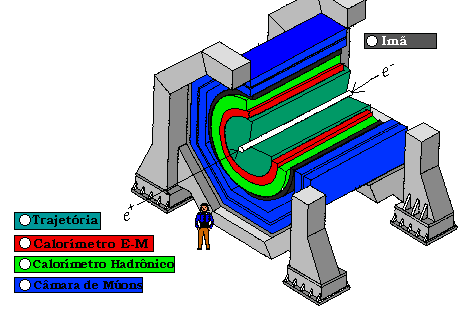
\includegraphics[scale=0.7]{modern_detect}
\end{center}
\caption{O diagrama de um detetor cilíndrico moderno.}
\label{fig:modern-detect}
\end{figure}

Na Figura~\ref{fig:modern-detect}, é possível observar que um detetor moderno
é composto, basicamente, de 4 sub-detetores principais. O primeiro detetor, de
dentro para fora (tomando o feixe de partículas como origem), tem a função de
determinar a rota e curvatura de partículas, por isto é chamado de detetor de
trajetória, arrasto ou, mais comumente, traços. A curvatura das partículas
sobre o campo magnético a que são expostas no detetor dá informações sobre a
carga da partícula e seu momento. O segundo detetor é chamado calorímetro
eletromagnético (e.m.) e tem a função de determinar a energia total de
elétrons, pósitrons e fótons (raios $\gamma$). Estas partículas interagem com
este detetor, originando chuveiros compostos de outros elétrons, pósitrons e
fótons. O terceiro detetor, o calorímetro hadrônico, mede a energia total de
chuveiros originados por hádrons (prótons, nêutrons ou mésons). No caso de
partículas hadrônicas, este chuveiro é bastante mais largo e profundo que o
equivalente para partículas como elétrons e fótons. O quarto detetor é um
detetor de múons. Somente estas partículas e neutrinos escapam dos outros
sistemas de deteção. Neutrinos, infelizmente, nem por este último são
detetados. Sua massa pode ser estimada, no entanto, através da energia
faltante no evento \cite{atlas-tp}. A Figura~\ref{fig:decay} mostra como
alguns tipos de partículas interagem com estes detetores. Fótons, por exemplo,
têm carga nula e não são detetados pelos detetores de traços, mas interagem
com os calorímetros e.m.. Elétrons e pósitrons interagem tanto com os
detetores de traços quanto com o calorímetro e.m., desenvolvendo cascata
e.m. neste último. Prótons são detetáveis pelos detetores de traços, mas
desenvolvem cascata somente nos calorímetros hadrônicos. Nêutrons somente
desenvolvem cascata nos detetores hadrônicos.

\begin{figure}
\begin{center}
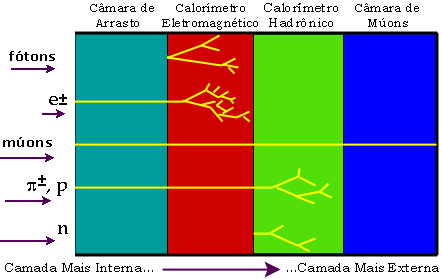
\includegraphics[scale=0.6]{decay_chart}
\end{center}
\caption{A interação de partículas com os detetores modernos.}
\label{fig:decay}
\end{figure}

\section{Calorimetria Moderna}
\index{Calorimetria}
\label{sec:calorimetria}

Geralmente, \idx{calorímetros} são detetores compostos utilizando a absorção
total de partículas para medir a energia e a posição de partículas e
jatos. Durante o processo de absorção, chuveiros são gerados por cascatas de
interações. Durante a formação do chuveiro, eventualmente, a maior parte da
massa da partícula será convertida em radiação ionizante, o que explica o nome
deste tipo de detetor. É claro, nenhuma temperatura é medida, mas as
características de interação com a matéria (e.g. excitação atômica, ionização)
são utilizadas para gerar um efeito detetável, através de partículas
carregadas. A calorimetria é também uma forma previsível de medir partículas
neutras entre as secundárias produzidas em uma colisão de altas energias
\cite{bock:detector, booth}.

Estes detetores são normalmente compostos de diferentes partes e têm seu
desempenho otimizado para as diferentes partículas que incidirão sobre seu
corpo. Cada calorímetro é feito de múltiplas \idx{células} individuais, sobre
o qual o volume, a energia absorvida, é integrada. As células são alinhadas
para formar torres tipicamente na direção de incidência. A análise da energia
depositada nas células e torres permite medir o perfil lateral e longitudinal
das cascatas e daí sua geometria ser otimizada para este propósito.

Tipicamente, \idx{partículas eletromagnéticas} incidentes (i.e. elétrons e
fótons) são completamente absorvidos em calorímetros eletromagnéticos, a
primeira das camadas de calorímetros compostos. Sua construção aproveita-se da
geometria de chuveiros eletromagnéticos que são compactos e curtos para medir
a energia e posição com precisão ótima para estas partículas, que incluem
$\pi^{0}$'s, decaindo eletromagneticamente.

\idx{Hádrons} incidentes (prótons, nêutrons, etc.), diferentemente,
podem começar seu decaimento no calorímetro eletromagnético, mas quase sempre
somente serão completamente absorvidos em camadas posteriores, i.e. em
\idx{calorímetros hadrônicos}, construídos exatamente para conterem estes
chuveiros. Chuveiros hadrônicos têm formato bastante diversificado.

A discriminação, comumente executada no sistema de filtragem do experimento
(veja a Seção~\ref{sec:trigger}), entre chuveiros eletromagnéticos e
hadrônicos, é um critério importante para um calorímetro. Portanto, é
importante conter chuveiros eletromagnéticos em um espaço mais curto, sem que
se inicie um grande número de chuveiros hadrônicos.

Calorímetros também provêm assinaturas para partículas que não são absorvidas:
\idx{múons} e \idx{neutrinos}. Múons não formam chuveiro na matéria, mas sua
carga deixa um sinal de ionização, que pode ser identificado em um
calorímetro se a partícula está suficientemente isolada (e a eletrônica
associada permitir), e então pode ser associada a um traço detetado nos
detetores de traço ou no detetor de múons. Neutrinos, por outro lado, não
deixam sinais em um calorímetro, mas sua existência pode ser algumas vezes
inferida através do princípio da conservação de energia: num calorímetro
hermeticamente fechado, ao menos um neutrino suficientemente energético ou
grupo desbalanceado de neutrinos pode ser observado formando-se a soma
vetorial de todos os outros momentos medidos, tomando a energia observada em
cada célula do calorímetro. A precisão de tais métodos, usualmente limitada à
direção transversal, requer um vazamento mínimo de energia em todas as
direções e daí o desafio para o projeto de calorímetros na prática.

\subsection{Tipos de Calorímetros}

Quanto à construção, é possível distinguirem-se os seguintes tipos de
calorímetro \cite{bock:detector, hadcal}:

\begin{itemize}
  \item \textbf{Homogêneos:}\index{Calorímetro!Homogêneo} Em calorímetros
  deste tipo, as funções de absorção e geração e leitura de sinais são
  combinadas em um único tipo de material. Estes materiais são quase que
  exclusivamente usados para calorímetros eletromagnéticos, por exemplo
  cristais, materiais compostos ou gases nobres em estado líquido;

  \item \textbf{Heterogêneos:}\index{Calorímetro!Heterogêneo} Tam\-bém
  conhecidos como \idx{ca\-lo\-rí\-me\-tros de amostragem}. Neste tipo de
  detetor, as fun\-ções de ab\-sor\-ção de energia e leitura do sinal são
  separadas. Isto permite uma escolha ótima do material de absorção e
  liberdade no tratamento do sinal. Calorímetros heterogêneos são, em sua
  maior parte, construídos como sanduíches (e.g. aço, ferro e urânio),
  alternando estes materiais com camadas de material ativo (e.g. cintiladores
  líquidos, sólidos ou contadores proporcionais). Somente parte da energia do
  chuveiro absorvida pelo material ativo é medida. Calorímetros hadrônicos,
  necessitando de uma profundidade considerável e largura para criar e
  absorver os chuveiros, são necessariamente deste tipo (veja a
  Seção\ref{sec:calohad}).

  Ainda que o desempenho não dependa fortemente da orientação, a espessura não
  pode variar em demasiado para assegurar uma resolução independente da
  direção e da posição dos chuveiros.
\end{itemize}

A calorimetria moderna é a arte de escolher entre duas restrições
conflitantes; a principal é normalmente formulada em termos da resolução em
energia, coodernadas espaciais, capacidade de filtragem, dureza à radiação dos
materiais usados e em parâmetros eletrônicos como a faixa de operação e a
extração de sinais. Na maior parte dos casos, o custo final de produção, a
segunda restrição, é o parâmetro mais limitante. O número de soluções em
calorimetria é maior para calorímetros do que para detetores de traços, e
soluções bastante engenhosas foram encontradas nos últimos 15 anos
\cite{hadcal}.

\subsection{A Física da Calorimetria}

A acurácia das medidas de energia em calorímetros aumenta com o aumento da
energia de partículas incidentes \cite{hadcal}, de acordo com a fórmula
empírica:

\begin{equation}
  \frac{\sigma_{E}}{E} \approx \frac{a}{\sqrt{E}} + b
\end{equation}

Onde $E$ é a energia da partícula incidente e $\sigma_{E}$ representa o desvio
padrão da medida de energia e $a$ e $b$ são constantes que dependem do tipo de
detetor, e.g. sua espessura e características das camadas ativas e passivas.

\subsubsection{Calorimetria eletromagnética}
\index{Calorimetria!eletromagnética}

Partículas eletromagnéticas perdem energia através de dois processos durante a
interação com calorímetros:

\begin{itemize}
\item {\bf radiação:} através do fenômeno conhecido como
  \idxeng{Bremsstrahlung}, onde a partícula incidente muda de rota, perdendo
  energia e gerando um fóton. Este fóton seguirá um caminho de interação
  independente do elétron original, possivelmente através de espalhamento
  Compton, efeito foto-elétrico ou produção de pares elétron-pósitron,
  dependendo diretamente da energia com o qual foi gerado. Os elétrons
  remanescentes deste processo, se tiverem energia, poderão repetir este
  processo até que as partículas formadas não possam mais irradiar. Esta
  energia limite é conhecida como \idx{Energia Crítica} ($\varepsilon_{c}$) e
  depende do peso atômico (Z) do material por onde se desenvolve a cascata
  eletromagnética. Valores típicos de $\varepsilon_{c}$ estão na faixa de
  dezenas de MeV (exemplo: $\varepsilon_{c}(Cu) = 25$ MeV). Quanto maior o
  número atômico, maiores as chances de perda por radiação\cite{knoll, leo}.

\item {\bf ionização:} interagindo com o núcleo do material em que viaja a
  partícula, ionizando-o e desta forma perdendo energia. Este fenômeno é mais
  contido longitudinalmente se comparado ao anterior.
\end{itemize}

Por estas razões, chuveiros eletromagnéticos são curtos e bem contidos em
calorímetros pouco espessos. A cascata desenvolve-se do traço gerado pela
par\-tí\-cu\-la que penetra no calorímetro de forma aproximadamente
isotrópica, num espaço de tempo extremamente curto, na ordem de centenas de
picossegundos.

A Figura~\ref{fig:cms-ecal} mostra um diagrama esquemático em três dimensões
da seção eletromagnética do calorímetro do experimento \idx{CMS} (do inglês
\idxeng{Compact Muon Solenoid}) no CERN, Suíça. Este calorímetro em formato
cilíndrico é feito de cristais compostos. Na cavidade central deste aparato
encaixam-se os detetores de traço do experimento. A segmentação do detetor é
indispensável para a localização de objetos no espaço.

\begin{figure}
\begin{center}
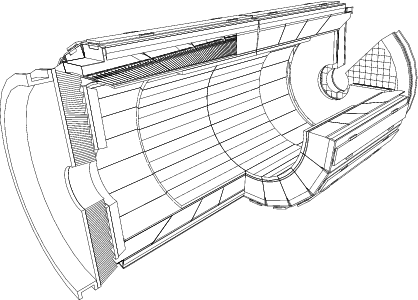
\includegraphics[scale=0.8]{cms-ecal}
\end{center}
\caption{Diagrama da seção eletromagnética do calorímetro do experimento CMS.}
\label{fig:cms-ecal}
\end{figure}

\subsubsection{Calorimetria hadrônica}
\index{Calorimetria!hadrônica}
\label{sec:calohad}

O chuveiro hadrônico é dominado por uma sucessão de interações hadrônicas
inelásticas. Em altas energias, estas são caracterizadas pela produção de
partículas múltiplas e pela emissão de partículas originárias de decaimentos
nucleares do material excitado. Devido a freqüente geração de $\pi^{0}$'s
(diz-se ``pi-zeros'', ou seja, píons que não possuem carga elétrica),
chuveiros hadrônicos têm também componentes eletromagnéticas.

Quando um hádron altamente ener\-gé\-tico penetra num bloco de ma\-té\-ria,
ele, em algum ponto, interagi\-rá com algum nú\-cleo atômico. Neste processo,
mésons são usualmente gerados (píons, káons, etc.). Outra fração da energia
inicial da partícula é transferida para o núcleo com o qual o hádron
interagiu. Este núcleo excitado, liberará esta energia emitindo um certo
nú\-mero de nú\-cleons (prótons ou nêutrons) e num estado posterior,
$\gamma$'s de baixa energia, perdendo sua energia cinética por ionização. As
partículas produzidas nesta reação (mésons, núcleons e $\gamma$'s), por sua
vez, podem perder sua energia cinética por ionização ou induzir novas reações
formando uma cascata ou chuveiro \cite{hadcal}.

Limites intrínsecos na resolução em energia de calorímetros hadrônicos são
\cite{hadcal}:

\begin{itemize}
  \item Uma componente $\pi^{0}$, flutuante dentre os chuveiros secundários, que
  interaja eletromagneticamente sem qualquer outra interação nuclear ($\pi^{0}
  \rightarrow \gamma\gamma$). A fração de $\pi^{0}$'s é dada por
  $\frac{\pi^{0}}{all} \approx 0,10 \log{E}$, $E$ em GeV. Chuveiros hadrônicos
  podem desenvolver uma componente eletromagnética dominante;

\item Uma boa parte da energia disponível é convertida em excitação e quebra
  de núcleos atômicos. Somente uma pequena fração desta energia aparecerá como
  sinal detetável, havendo largas flutuações evento-a-evento. Estas flutuações
  podem ser compensadas com a boas escolhas dos materiais ativos e absorvedores
  do detetor;

\item Uma fração considerável da energia da partícula incidente é despendida
  em reações que não resultarão em sinal observável, tais como vazamento de
  energia em várias formas (evaporação ou quebra nuclear, excitação nuclear,
  etc.).
\end{itemize}

De forma contrária a chuveiros eletromagnéticos, que se desenvolvem num curto
espaço de tempo, a física de chuveiros hadrônicos é caracterizada por
diferentes escalas de tempo. Os fenômenos mais lentos podem durar de centenas
de nanossegundos a um microssegundo.

Resumindo as razões pelas quais os calorímetros emergiram como detetores-chave
em praticamente todos os experimentos em física de partículas encontramos:

\begin{enumerate}
\item Calorímetros são sensíveis a partículas neutras e carregadas;

\item Devido a diferenças na forma de deposição de energia das partículas, a
identificação de partículas com alta eficiência pode ser atingida usando-se
calorímetros;

\item Quanto maior a energia da partícula, mais acurado é o resultado. Isto não
acontece com outros tipos de detetores;

\item Para conter o desenvolvimento de cascatas dos objetos a serem medidos, a
profundidade dos calorímetros aumenta logaritmicamente com a energia, o que
permite o projeto de detetores mais compactos;

\item Não precisam de campos magnéticos (como os detetores de traços);

\item Podem ser segmentados, o que permite acurada medida da energia e a
visualização da tra\-je\-tó\-ria das par\-tí\-cu\-las;

\item Resposta rápida (melhor que 50 ns) pode ser atingida, o que é importante
num ambiente com alta taxa de eventos;

\item A informação de energia pode ser usada para filtrar eventos interessantes
com alta seletividade;
\end{enumerate}

\section{Sistemas de Filtragem}
\index{Sistemas de Filtragem}
\label{sec:trigger}

Os sinais detetados por calorimetria são normalmente utilizados como fonte de
discriminação rápida de eventos interessantes em experimentos modernos. Um
Sistema de Filtragem, ou \idxeng{Trigger}, é um conjunto de dispositivos,
normalmente uma combinação de componentes eletrônicos e computadores, provendo
um sinal rápido quando a física interessante acontece
\cite{cms-trigger, d0-trigger, d0-trigger2, hlt-tdr, trig-review,
bock:detector}. Tipicamente, um sistema de filtragem está associado a
experimentos com detetores e seus sinais ativam o sistema de gravação de
eventos para registrar parte ou a totalidade dos impulsos captados em mídia
permanente. As condições que levam o sistema de filtragem a produzir o sinal
de aceitação são comumente chamadas de
\idx{assinaturas do evento}. As condições podem ser tão simples quanto
identificar um traço gerado por uma partícula carregada passando por
cintiladores durante um período de tempo, ou tão complexos quanto o critério
de massa efetiva entre léptons identificados que devam satisfazer colisões de
altas energias.

Em muitos experimentos, a aquisição de dados, através do \idx{tempo morto} que
causa, é um fator crítico determinante, que limita as estatísticas e o
potencial físico. Um sistema de filtragem eficaz é então o ponto-chave para a
transmissão de dados que têm alta probabilidade de conter física de interesse
e rejeição, com base nas possibilidades de deteção, de todos ou da maioria dos
eventos que representem física ordinária e trivial. Claramente, não somente a
eletrônica e informática do sistema de filtragem são necessárias ao trabalho,
mas também os dados carregados pelo sistema de leitura do detetor, que provêm
as informações que serão averiguadas pelo primeiro.

Dependendo do acelerador utilizado, sistemas de filtragem podem ser chaveados
(e.g. por pacotes de partículas chegando ao ponto de colisão) ou
permanentemente ativados (como para o estudo de raios cósmicos). As
implementações podem ser síncronas ou operar em tempo real, ou ainda
se comporem de vários circuitos assíncronos operando paralelamente,
respeitando uma unidade de controle central (que também tem a função de
re-sincronizar o sistema como um todo). As implementações nos dias de hoje vão
desde simples portas E/OU até \idxeng{Field-Programmable Gate Arrays} ou
\idx{FPGA}'s. Os tempos de retardo dependem do volume dos dados a serem
analisados (e comumente na ocupação de recursos locais). Algoritmos de
filtragem também podem ter seu tempo de execução dependente do tempo já que
variam com a complexidade dos cálculos envolvidos.

Em grandes experimentos, sistemas de filtragem são implementados em múltiplos
níveis, tipicamente consistindo de um primeiro nível assíncrono, que identifica
candidatos a partir de um subconjunto dos dados colhidos pelos detetores,
reduzindo a taxa de eventos por algum fator. Subseqüentemente, os dados são
digitalmente transmitidos para \idx{bancos de memória} (do inglês
\idxeng{buffers}) e para um segundo nível de filtragem, normalmente assíncrono,
onde algoritmos mais complexos, baseados em um conjunto de dados mais completo
conseguem reduzir novamente a taxa de eventos. Eventualmente, depois, talvez,
de uma terceira ou quarta iteração, o evento é gravado em mídia permanente.

As implementações de sistemas de filtragem não somente dependem do projeto do
detetor e da forma com que seus dados são lidos, mas também da tecnologia de
transmissão de dados que se desenvolve tão rapidamente nos dias de hoje. As
comparativamente complexas situações de fluxo de dados podem somente ser
compreendidas utilizando-se programas de modelagem ou \idx{simulações de Monte
Carlo}. A teoria de filas permite a predição do comportamento a nível local
nos nós de processamento do sistema.

\subsection{Sistemas de filtragem em experimentos modernos}

Um experimento em Física de Altas Energias como o DZERO \cite{d0}, localizado
no FermiLab, próximo a Chicago nos Estados Unidos, faz um bom exemplo de um
experimento com um sistema de filtragem moderno. O cruzamento de pacotes de
prótons e anti-prótons que geram as colisões a serem estudadas ocorrem numa
taxa de 2,5 MHz (ou seja, 2,5 milhões de colisões por segundo). Cada colisão
poderá produzir um evento que possui 0,25 \eng{megabytes} em dados. Se a taxa
total fosse escrita em fitas magnéticas, assumindo um custo de 40 centavos de
dólar por \eng{Gigabyte}, o custo total seria de 10,5 milhões de dólares por
ano. No entanto, a maior parte das colisões de pacotes contém interações
fracas ou até mesmo nulas. Para tirar proveito desta natureza, o experimento
DZERO emprega um sistema de filtragem em múltiplos níveis para reduzir a taxa
de eventos registrada a 50 Hz, implicando em um custo aproximado de 75.000
dólares por ano em fitas magnéticas.

É claro que a economia em fitas magnéticas não são a única razão da existência
de um sistema de filtragem. Planejar e projetar um sistema de aquisição de
dados com uma banda passante de 600 \eng{gigabytes} por segundo seria
proibitivo economicamente, especialmente considerando-se o valor relativo dos
dados coletados. Os programas de reconstrução de eventos atuais também
consomem mais e mais poder de processamento e, se a entrada puder ser
sensivelmente reduzida em volume, menor a quantidade de recursos
computacionais serão necessários.

O enfoque usado para projetar e implementar um sistema de filtragem depende
fortemente do domínio do problema. Um experimento moderno em Física de Altas
Energias deve estar apto a responder a um novo evento, num geral, a cada
dezena ou dezenas de nanossegundos. O \idx{tamanho do evento} para grandes
experimentos (veja a Figura~\ref{fig:eventsize}) também tende a ser grande,
chegando a alguns
\eng{megabytes} por evento em alguns dos experimentos do \idx{LHC}
(\idxeng{Large Hadron Collider}).

\begin{figure}
\begin{center}
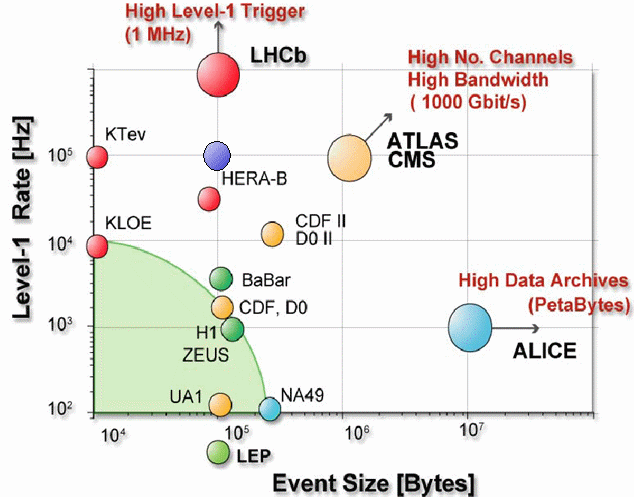
\includegraphics[scale=0.6]{eventsize}
\end{center}
\caption{O tamanho do evento \eng{versus} a taxa de produção em experimentos
atuais.}
\label{fig:eventsize}
\end{figure}

Experimentos modernos usam um sistema de filtragem dividido em múltiplos
níveis para endereçar o problema das taxas de entrada. Os níveis mais baixos
implementam algoritmos simples e rápidos, normalmente usando FPGA's e
\eng{hardware} personalizado, que removam \eng{backgrounds} mais simples e
abundantes. Os níveis mais altos são progressivamente mais sofisticados e
também requerem mais tempo para atingir níveis de rejeição
aceitáveis. Ademais, carregando uma menor quantidade ou qualidade de dados nos
níveis iniciais de filtragem, estes experimentos conseguem reduzir o fluxo de
informação no sistema de leitura: tão pronto um evento seja rejeitado, seus
dados são descartados.

Classicamente, o nível em \eng{hardware} é chamado de \idx{Primeiro Nível}. O
seguinte, compondo de partes personalizadas em \eng{hardware} e computadores,
é chamado de \idx{Segundo Nível}. O último estágio, chamado de
\idx{Terceiro Nível}, composto normalmente de redes de computadores
domésticos, realiza a classificação final. Comumente o segundo e terceiro
níveis de filtragem são conhecidos como \idx{Filtros de Alto Nível} ou
\idxeng{High-Level Triggers}, \idx{HLT}.
